\chapter{Introduction}
\section{Artificial Neural Networks}

Artifical Neural Networks (ANNs) are a very popular machine learning model. They are known to be very expressive, leading to low statistical bias. With enough neurons, ANNs can approximate any function, also known as the Universal Approximation Theorem\cite{cybenko1989}.  They are especially useful for learning from very large data sets.

ANNs are composed of 'neurons', which are in some ways analogous to biological neurons.Each neuron is a nonlinear function transforming the weighted sum of its inputs and a bias:
\begin{equation}
      y = \sigma(w_1x_1+w_2x_2+...+w_nx_n + b)
\end{equation}

where $w$ are the weights, $x$ are the inputs to the neuron, which come either from a previous neuron, or are fed into the network, $\sigma$ is the activation function, and finally a bias $b$ is also added to the sum. This is the McCulloch-Pitts neuron model\cite{McCulloch1990}. The most commonly used activation function $\sigma$ is the Rectified Linear Unit (ReLU):

\begin{equation}
      \sigma(x) = x^+ = \max(0,x)
\end{equation}

Many other activation functions are possible, such as the sigmoid function ($\frac{1}{1+e^{-x}}$) or the hyperbolic tangent function ($\tanh(x)$). Figure \ref{sigmafig} plots the ReLU and $\tanh$ activation functions which are used in this thesis. Table \ref{sigprop} lists some properties of these functions. Particularly of interest is the fact that ReLU is not smooth everywhere, in $x=0$ the derivative is undefined \cite{wikiact}. In the code of this thesis it is taken to be $0$.


\begin{table}
\centering
\begin{tabular}{ c | c c c c}
Name & Function & Derivative & Range & Order of Continuity \\ \hline
ReLU & $\max(0,x)$ & $ 
     \begin{cases}
       0 &\text{if} \quad x \leq 0\\
       1 &\text{if} \quad x > 0 \\
     \end{cases}$ & $[0,\infty)$ & $C^0$ \\
Hyperbolic Tangent & $\tanh(x)$ & $\frac{2}{\cosh(2x)+1}$ & $(-1,1)$ & $C^{\infty}$
\end{tabular}
\caption{Properties of activation functions}
\label{sigprop}
\end{table}

\begin{figure}
	\centering
	\begin{subfigure}[b]{.49\textwidth}
		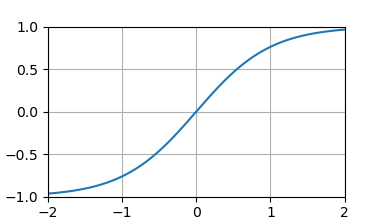
\includegraphics[width=\textwidth]{tanh}
		\caption{Hyperbolic tangent: $y = \tanh(x)$}
		\label{figtanh}
	\end{subfigure}
	%\caption{Feedforward Deep Neural Network. \cite}
	\begin{subfigure}[b]{.49\textwidth}
		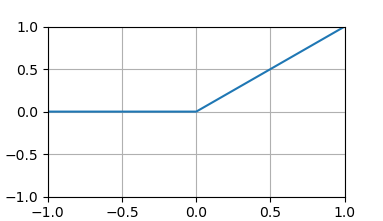
\includegraphics[width=\textwidth]{relu}
		\caption{ReLU: $y = x^+ = \max(x,0)$}
		\label{figrelu}
	\end{subfigure}
	\caption{Plot of two common activation functions}
	\label{sigmafig}
\end{figure}


A visual representation of a network is shown in figure \ref{neural:neur}. A full network is built by connecting layers of neurons as shown in figure \ref{neural:net}.

\begin{figure}[b]
	\centering
	\begin{subfigure}[b]{0.4\textwidth}
		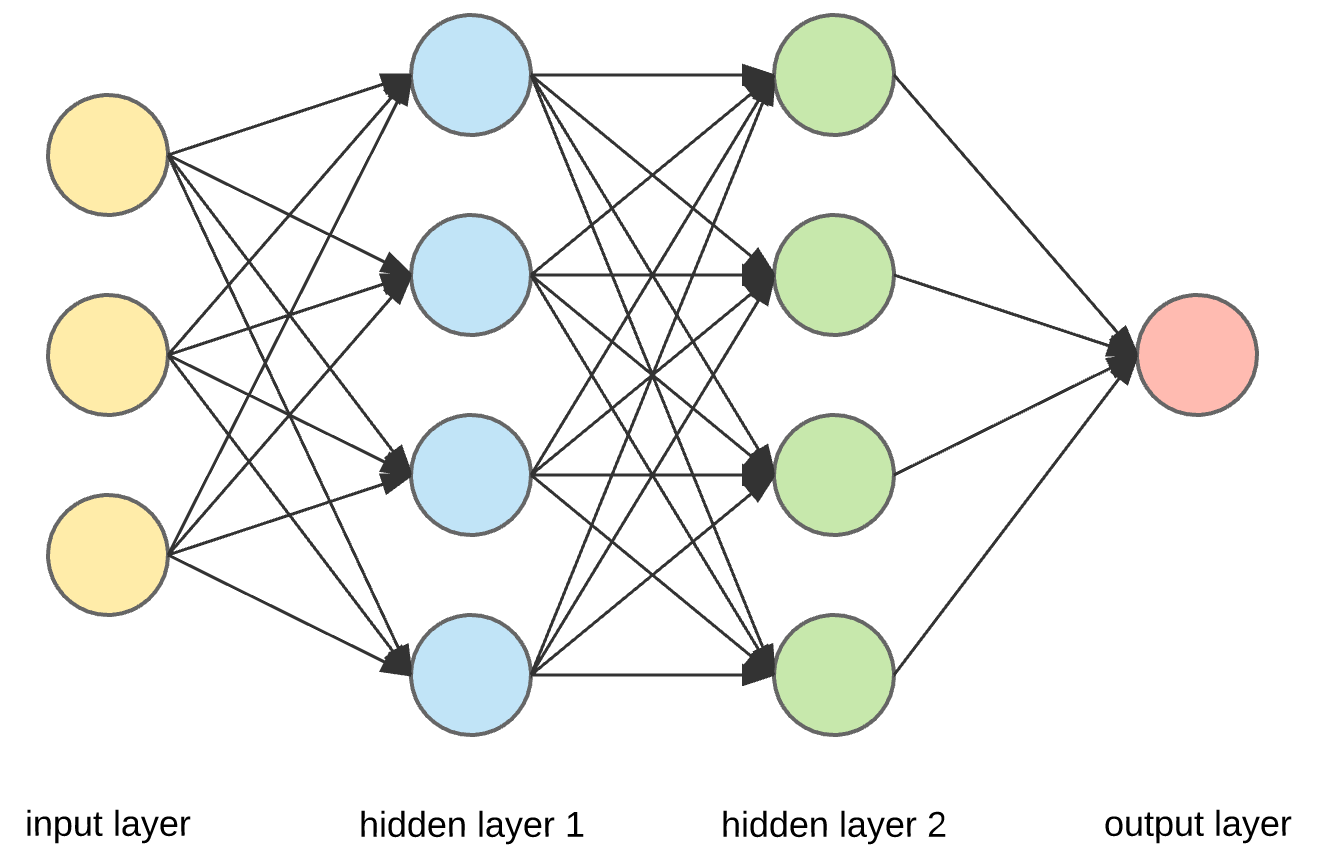
\includegraphics[width=\textwidth]{network}
		\caption{Deep Neural Network}
		\label{neural:net}
	\end{subfigure}
	%\caption{Feedforward Deep Neural Network. \cite}
	\begin{subfigure}[b]{0.4\textwidth}
		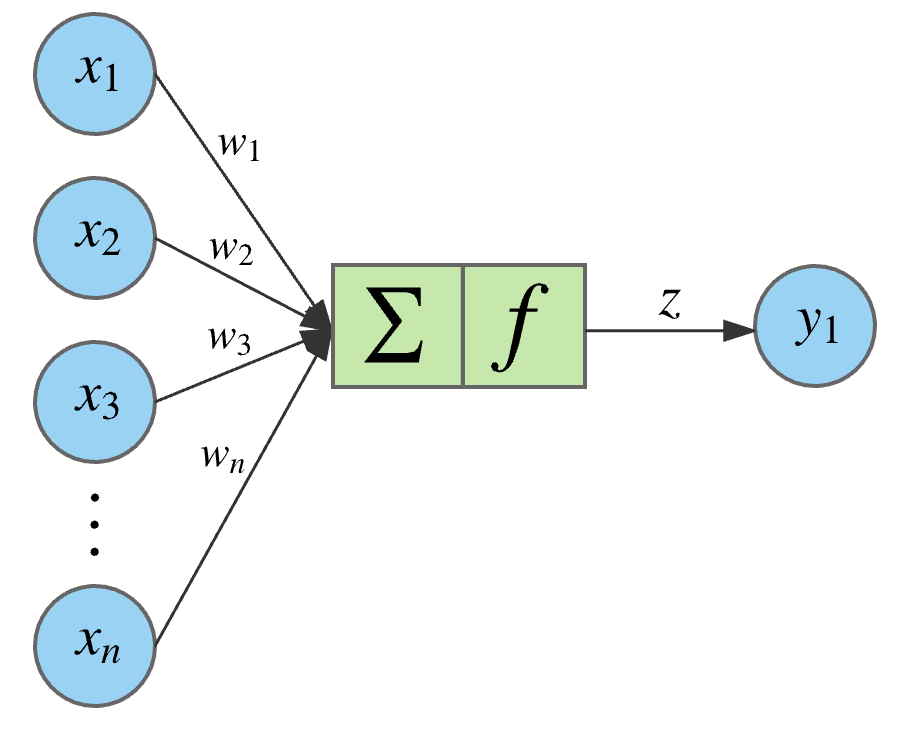
\includegraphics[width=\textwidth]{neuron}
		\caption{Single Neuron}
		\label{neural:neur}
	\end{subfigure}
	\caption{Feedforward Deep Neural Network and Single Neuron - McCulloch-Pitts model \cite{dertat2017}.}
	\label{neural}
\end{figure}

\section{Neural Network Training}
Training a neural network is an optimization problem as we will discuss in this section. However the theoretical understanding of ANN optimization is still quite limited. Quoting from \cite{jacot2020neural}: "... it is not known what the optimization of ANNs converges to. Indeed the loss surface of neural networks optimization problems is highly non-convex: it has a high number of saddle points which may slow down the convergence \cite{DauphinYann2014Iaat}". 

ANN training is a highly nonlinear problem, where most optimization algorithms can only arrive at a local minimum. The complexity of the loss surface means there can be a very large amount of local minima, which is an issue if these minima have a high cost compared to the global minimum, also known as the problem of "bad" local minima \cite{Goodfellow-et-al-2016}. This concept is difficult to define formally as finding the global minimum of a network is an intractible problem for practical networks. The problem of "bad" local minima was long feared to be a practical hurdle to good network training, but theoretical results \cite{ChoromanskaAnna2015Tlso},\cite{SaxeAndrewM2013Estt} suggest that this is uncommon for large neural networks. Many experts believe that for large networks, in practice, local minima have a low cost function, comparable to the global minimum \cite{Goodfellow-et-al-2016}. An interesting visualisation of the loss surface can be found in \cite{li2018visualizing}, figure \ref{surfvis} presents two graphics from this paper. The 3rd dimension represents the loss function, while the first two represent training parameters. It shows the non-convexity of the loss surface.

\begin{figure}
	\centering
	\begin{subfigure}[b]{.49\textwidth}
		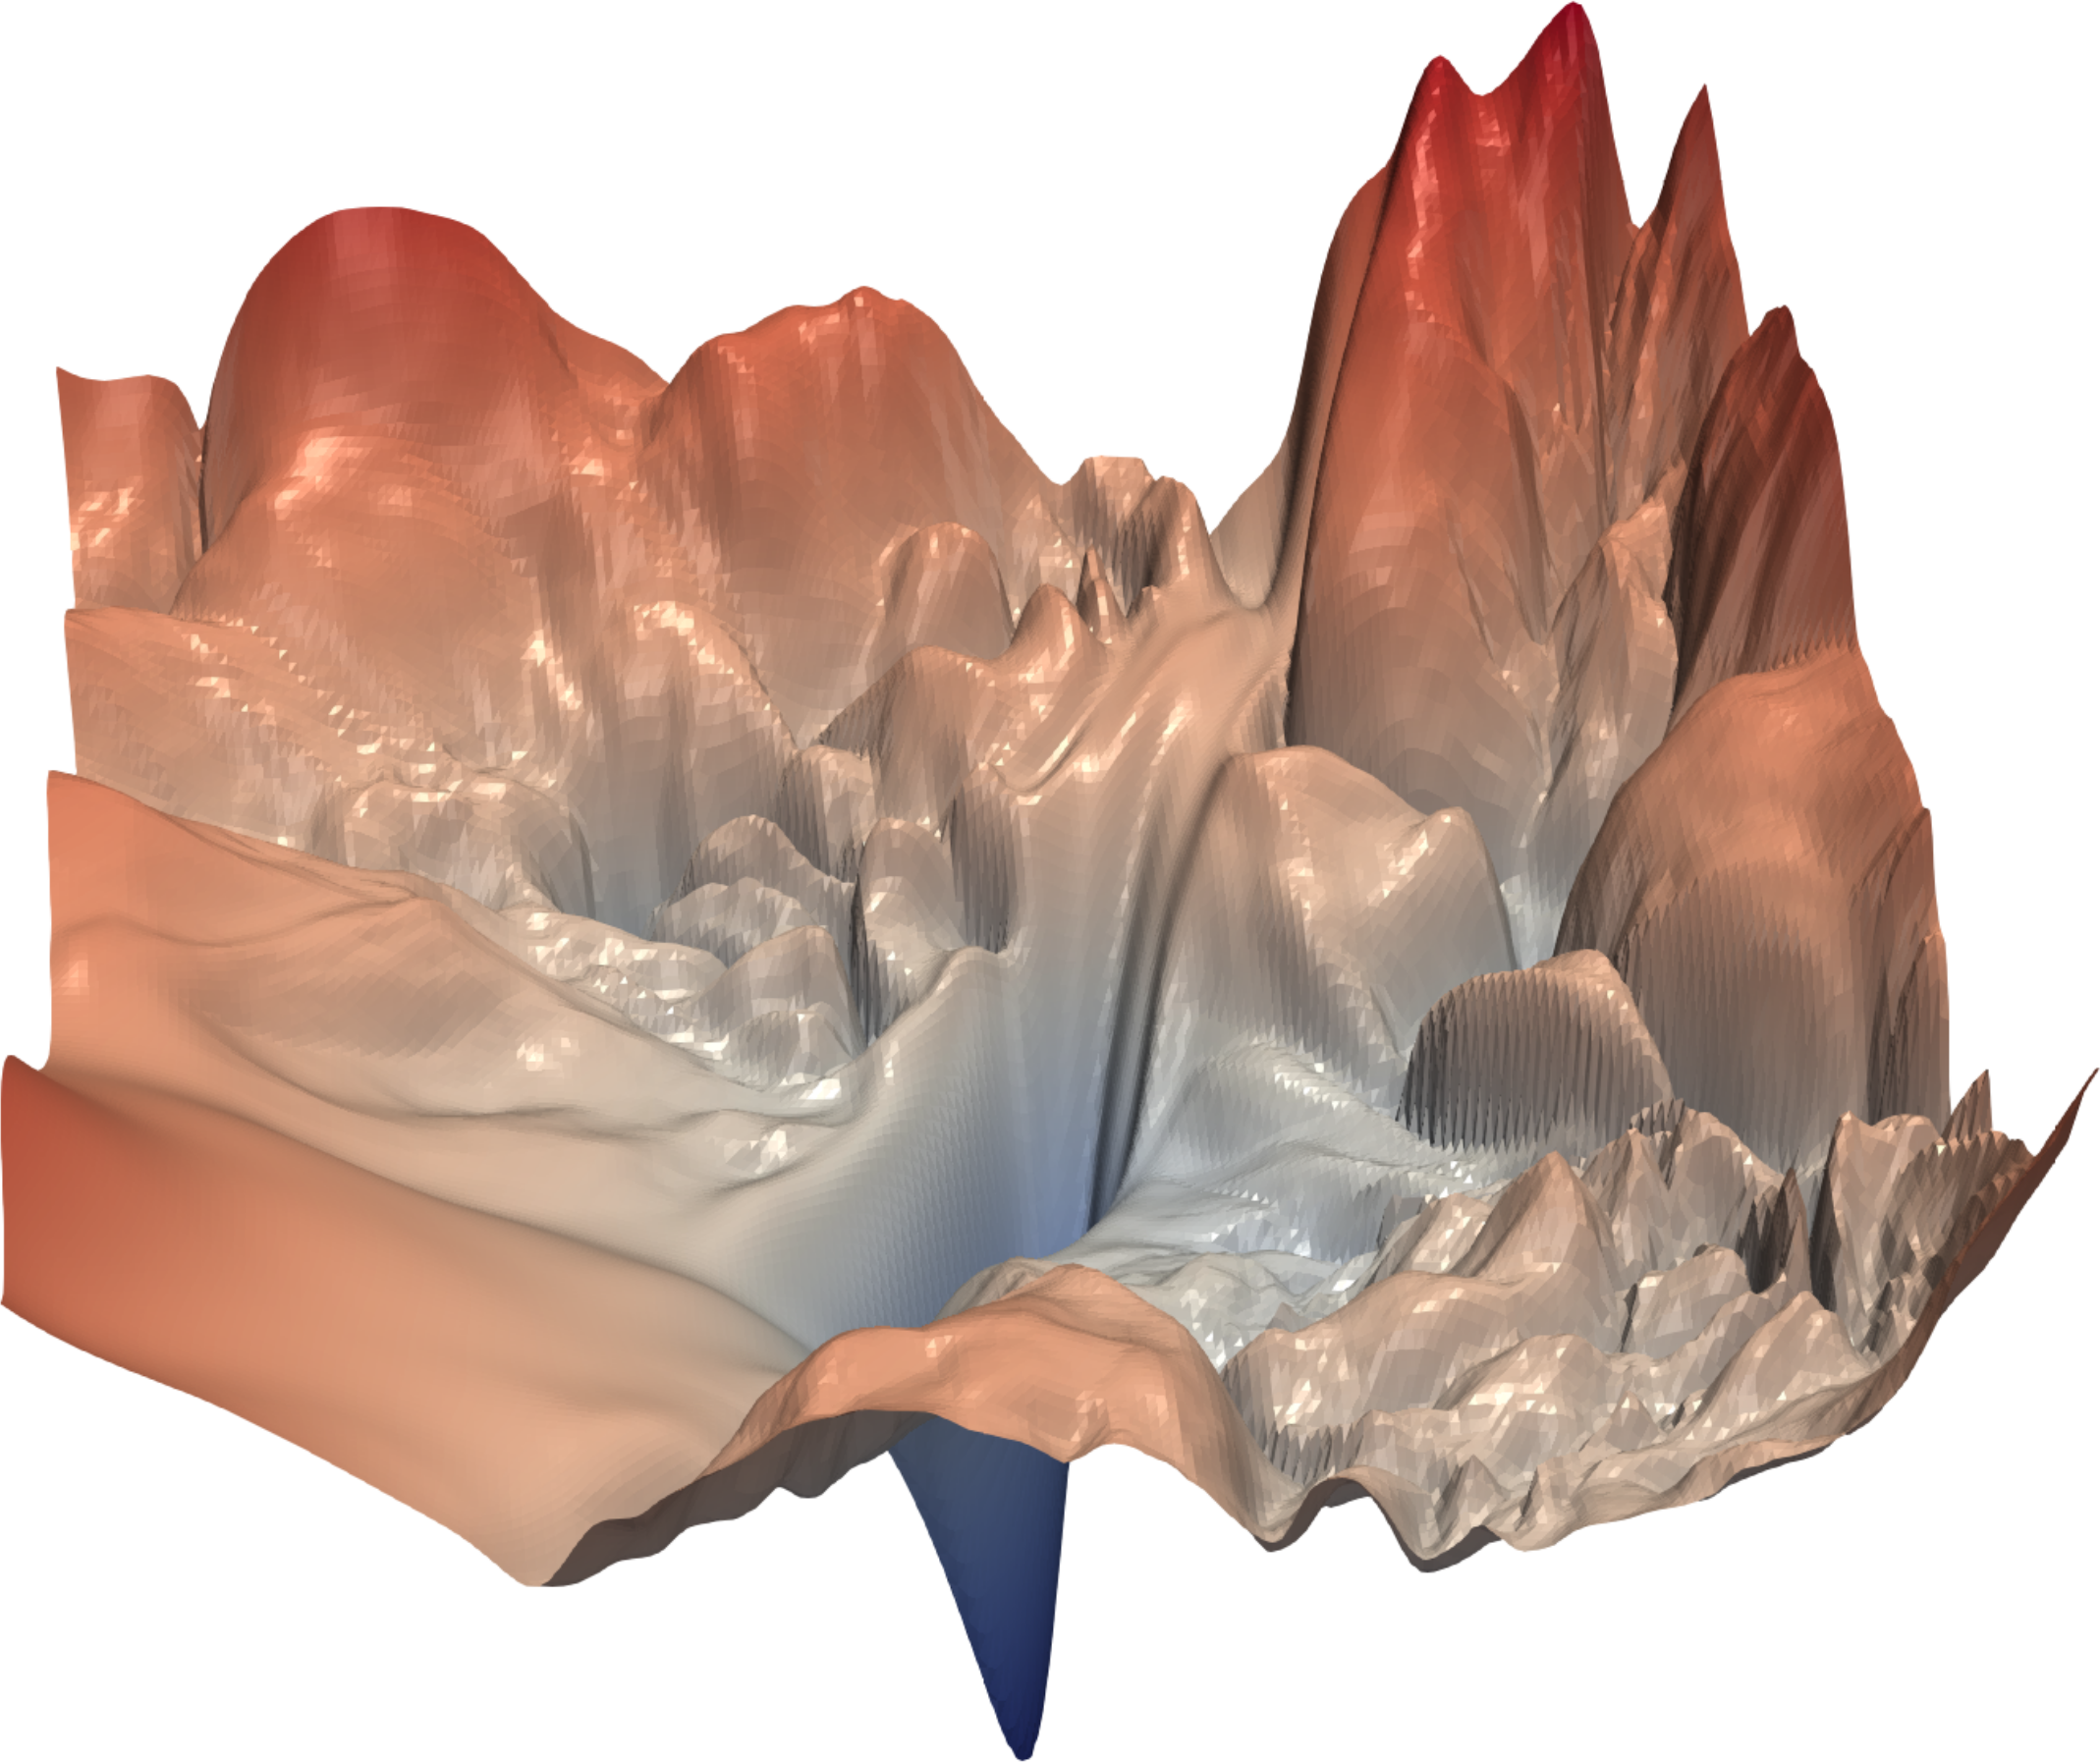
\includegraphics[width=\textwidth]{surface1}
		\caption{ResNet-56}
		\label{surf1}
	\end{subfigure}
	%\caption{Feedforward Deep Neural Network. \cite}
	\begin{subfigure}[b]{.49\textwidth}
		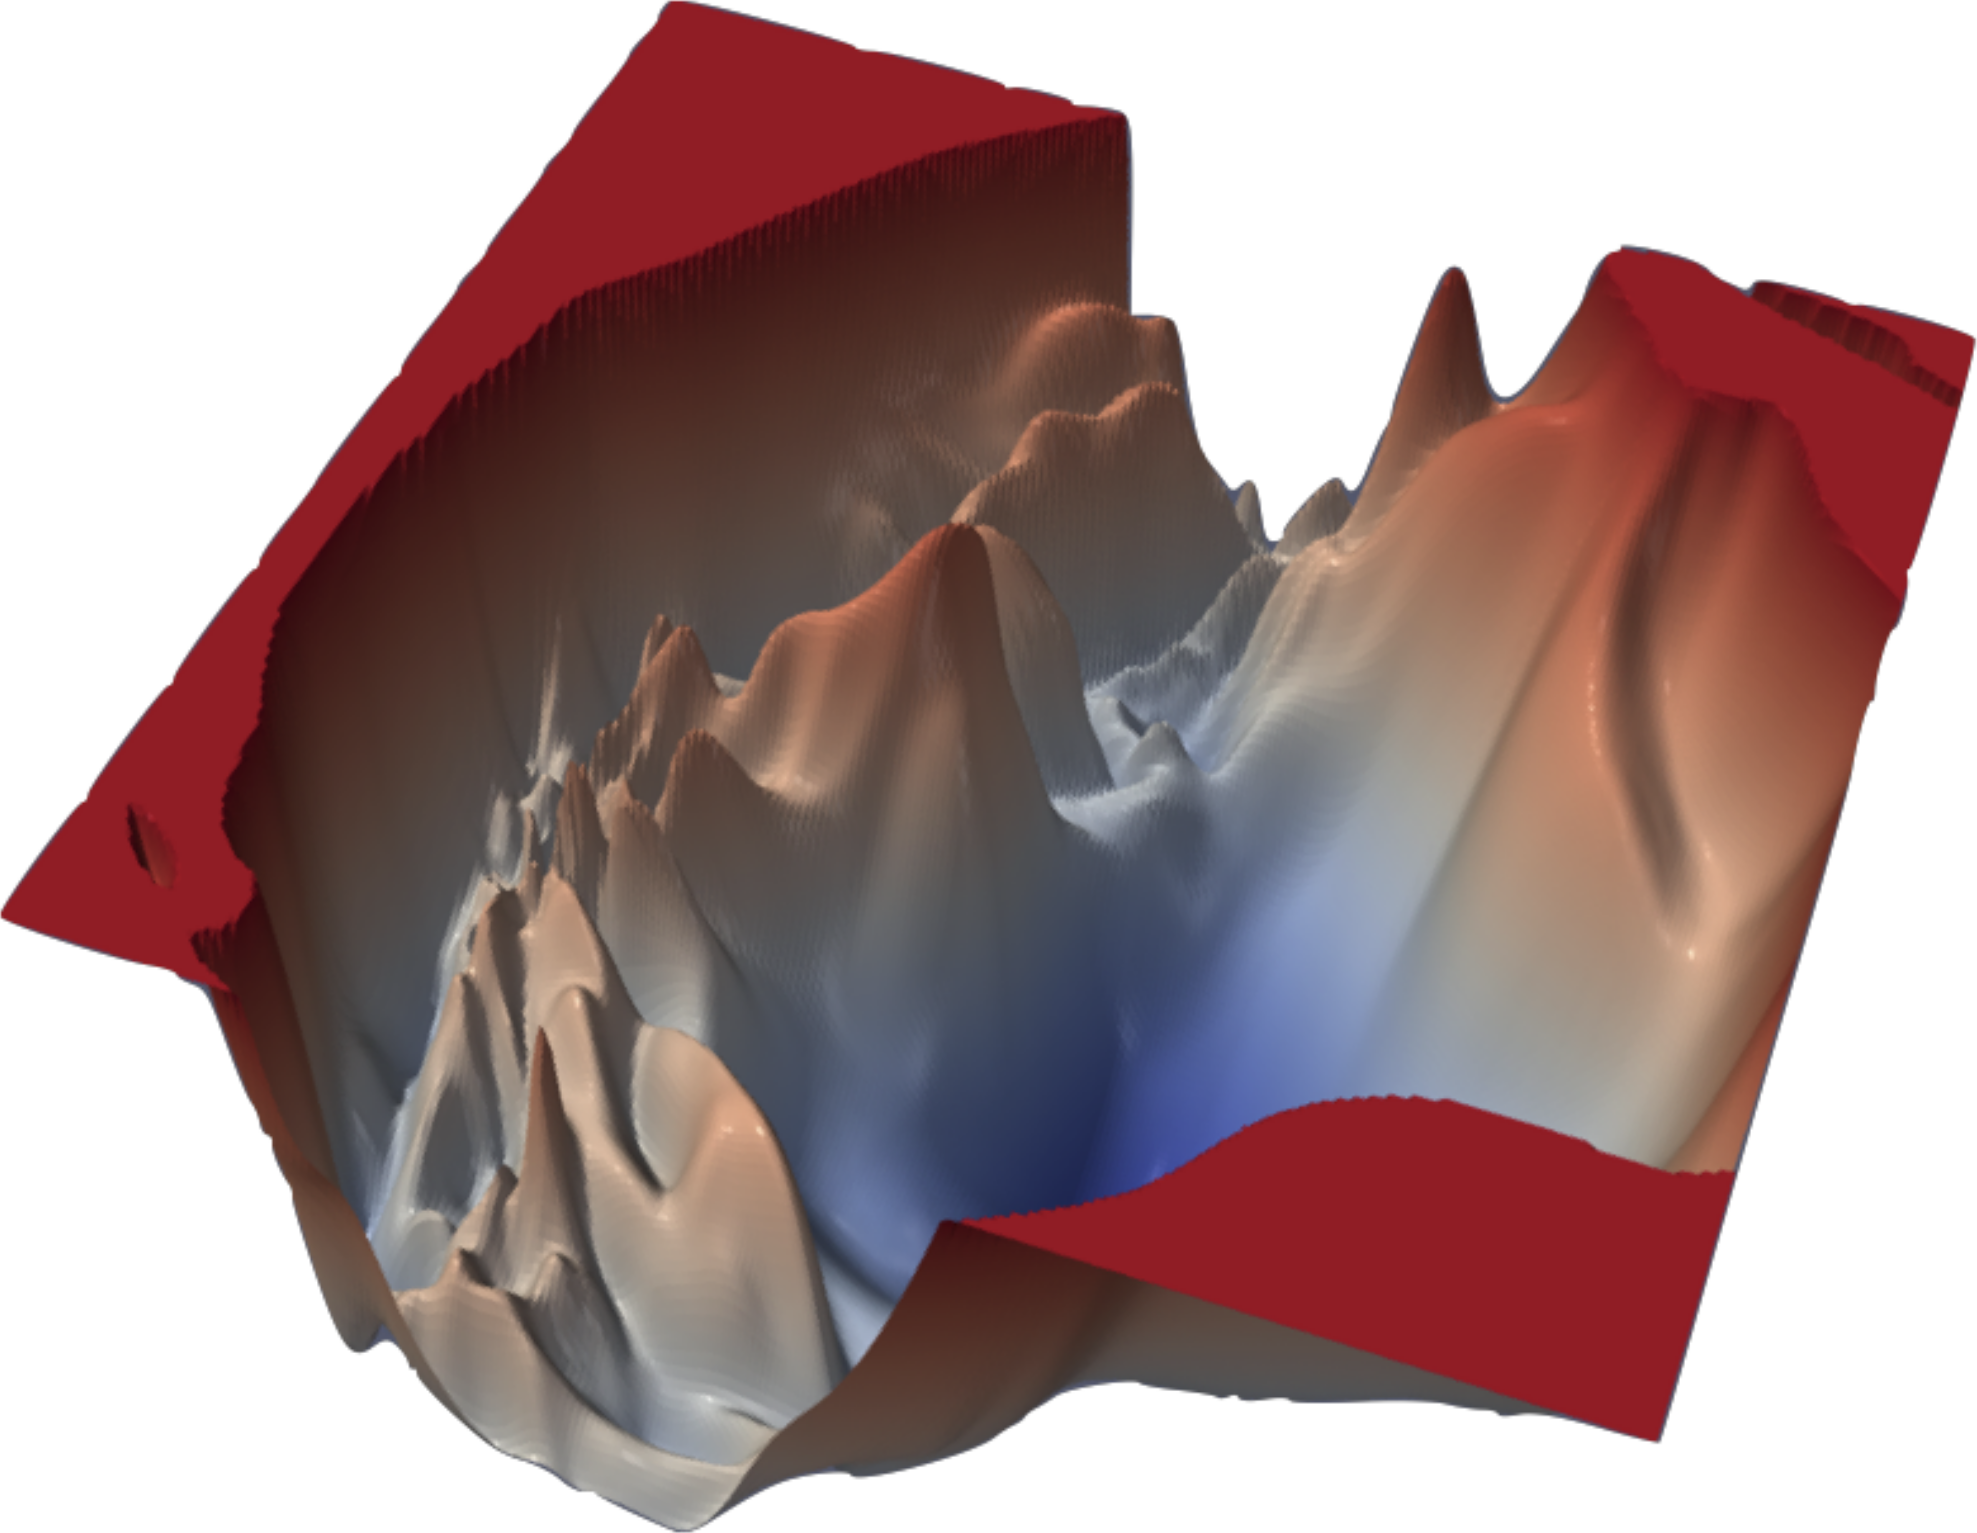
\includegraphics[width=\textwidth]{surface2}
		\caption{ResNet-110}
		\label{Surf2}
	\end{subfigure}
	\caption{Visualisation example of loss surface of neural network. Retrieved from \cite{li2018visualizing}.}
	\label{surfvis}
\end{figure}

Ruoyu Sun covers in \cite{sun2019optimization} the current theory and algorithms for optimizing deep neural networks, upon which much of this section is based.

In a supervised learning problem a dataset of inputs and desired outputs is given: $x_i \in \mathbb{R}^{d_x}, y_j \in \mathbb{R}^{d_y}, i = 1,\dots,n$ with $x_i$ the input vectors, $y_i$ the desired output vectors and $n$ the number of data points. We want the network to predict the output $y_i$ based on the information in $x_i$, i.e. we want the network to learn the underlying mapping that connects the data. A standard fully connected network can be expressed as a combination of function composition and matrix multiplication as follows:

\begin{equation}
         f_W(x) = \sigma_L(W_L\sigma(W_{L-1}\sigma_1(...W_1\sigma_0(W_0x)...)))
         \label{funeq}
\end{equation}

where $L$ is the number of hidden layers in the network and $\sigma_k$ is the activation function in each layer. In this equation, and also in the rest of the thesis, the bias vectors $b_k$ have been included in the weight matrixes:
\begin{equation}
W_k = \begin{bmatrix} W_{k,orig} & b_k \end{bmatrix}
\end{equation}
where $W_k$ are the matrixes of dimension $d_k \times (d_{k-1}+1), k=1 \dots L$ containing the connection weights extended with the bias vector $b_k$. Therefore the matrix multiplication in function \ref{funeq} implicitly also contains the operation of extending the input vector with a constant $1$ value. This simplifies the notation throughout the thesis

This function can also be defined recursively, which will be useful for later interpreting the network in an optimal control context.

\begin{equation}
	\begin{aligned}
	z_0 &= x \\
	z_{k+1} &= \sigma_k(W_kz_k), & k = 0,...,L \\
	f_W(x) &= z_{L+1} \\
	\end{aligned}
\label{st-eq}
\end{equation}

We want to pick the parameters of the neural network so that the predicted output $\hat{y}_i = f_W(x_i)$ is as close as possible to the true output $y_i$ for a certain distance metric $\mathit{l(\cdot,\cdot)}$. Thus the optimization problem can be written as follows:

\begin{equation}
\begin{aligned}
& \underset{W}{\text{minimize}}
& C(W) &= \sum\limits_{i=0}^{n}l(y_i,f_W(x_i)) \\
\end{aligned}
\label{op-eq}
\end{equation}

In this thesis only regression problems will be considered, where $l(x,y)$ is the quadratic loss function $l(x,y) = ||x^2-y^2||$, a.k.a. mean square error (MSE). 

For classification problems cross entropy loss is the most common cost function: $l(x,y) = x\log(y)+(1-x)\log(1-y)$, a. k. a. negative log-likelihood. This loss function is a proxy for the 0-1 loss which is commonly associated with classification problems. The advantage is that negative log-likelihood is a smooth function which can be optimized for. It also continues to decrease even after reaching 0, allowing the training to push the classes even further apart, making the network more robust.

Writing down equation \ref{op-eq} using the MSE gives the following optimization problem:

\begin{equation}
\begin{aligned}
& \underset{W}{\text{minimize}}
& C(W) &= \sum\limits_{i=0}^{n}||y_i - f_W(x_i)||^2_2 \\
\end{aligned}
\label{op2-eq}
\end{equation}

Most methods for solving equation \ref{op-eq} are based on gradient descent (GD). This algorithm uses the gradient of the loss function to search for a local minimum:

\begin{equation}
W_{k+1} = W_{k} - \eta_k\nabla F(W_k)
\label{gd-eq}
\end{equation}

where $\eta_k$ is the step size (a.k.a. "learning rate") and $\nabla F(W_k)$ is the gradient of the loss function at the $k$-th iterate.

In practice the datasets that are used in training can be large to very large, i.e. "Big Data". In these cases it is infeasible to calculate the gradient over all samples. Instead what is done is to calculate an approximation of the gradient over a small number of samples called a "mini-batch".

\begin{equation}
W_{k+1} = W_{k} - \eta_k\nabla^i F(W_k)
\label{gd-eq}
\end{equation}

where $\nabla^i F(W_k)$ is the gradient calculated with respect to the samples in the "mini-batch". In each epoch a different set of samples is selected. This is the Stochastic Gradient Descent method. In general this method will converge to the same solution \cite{Bottou2005}. This algorithm can be improved even further by using an adaptive learning rate $\eta_k$, such as RMSProp or ADAM. SGD methods with adaptive learning rate have emerged as the most effective algorithms in practice. The choice of which specific algorithm to use is largely based on the user's preference, and familiarity with the algorithm and its hyperparameters \cite{Goodfellow-et-al-2016}.

\section{Neural network training as an optimal control problem}
Neural network training can also be seen as an optimal control problem. A neural network is a multi-stage dynamical system, where every layer is a stage. The dynamics are ruled by the equations \ref{st-eq}. In optimal control the following objective cost function is considered:

\begin{equation}
E(\theta) = \sum\limits_{s=1}^{L-1}g^s(a^s,\theta^s) + h(a^L)
\end{equation}


$a^s$ and $\theta^s$ are the state and decision vectors at stage $s$, and $g^s$ and $h$ are the stage cost at stage $s$ and the terminal cost, respectively. In neural network training the stage costs are usually dropped. If the terminal cost is taken to be the MSE, the same cost function as in equation \ref{op2-eq} is found. The terminology and notation differences have been summarized in table \ref{trans-tbl}. Using neural network terminology the optimal control problem to be solved is the following:

\begin{equation}
	\begin{aligned}
	& \underset{W}{\text{minimize}}
	& & \sum\limits_{j=0}^{n}||\sigma_L(W_Lz_L) - y_j||^2_2 \\
	& \text{subject to}
	& & z_{1,j} = \sigma_0(W_0,x_j), &j = 1,\ldots,n \\
	& & & z_{k+1,j} = \sigma_k(W_kz_{k,j}), &k = 1,\ldots,L-1,j = 1,\ldots,n
	\end{aligned}
	\label{ocp-eq}
\end{equation}

This notation actually constructs $j$ parallel dynamical systems with the same weights, but different inputs, outputs and states. The cost function then concatenates them all together \cite{dreyfus1990}.

\begin{table}
\centering
\begin{tabular}{c | c | c | c}
Notation & Optimal Control & Neural Network & Notation\\ \hline
$\theta$ & decision variables & weight parameters & $W$\\
$a$ & state variables & (neuron) activation & $z$\\
& stage & layer \\
\end{tabular}
\caption{Comparison of notation between Control theory and Machine Learning}
\label{trans-tbl}
\end{table}


\section{Backpropagation}
The current standard algorithm for training a neural network is backpropagation (BP). It works by efficiently calculating the gradient for GD (equation \ref{gd-eq}). It was discovered and popularised in the context of neural networks by Rumelhart, Hinton \& Williams (1986) \cite{Rumelhart1986}. But it has been shown that by viewing the problem in an optimal control context, the backpropagation algorithm is the same as the gradient formulas discovered by Kelley and Bryson in 1960 \cite{dreyfus1990},\cite{kelley1960},\cite{Bryson1962}.

This section will explain how backpropagation works, it will largely follow and summarize \cite{Nielsen2015},\cite{wikiback}. Essentially BP evaluates the derivative of the cost function from the end to the front of the network, i.e. "backwards". It works on each input-output pair individually, with the full gradient given by averaging over all pairs.

Given an input-output pair $(x,y)$, the loss is:
\begin{equation}
C(y,W_L\sigma(W_{L-1}...\sigma(W_1\sigma(W_0x))))
\end{equation}
The loss is calculated forwards by evaluating the network, starting with the input $x$. Note the weighted input at each layer as $\nu_l = W_{l-1}z_{l-1} + b_{l-1}$. The activations $z_l = \sigma(\nu_l)$ and the derivatives $f'_l = \sigma'(\nu_l)$ at each layer $l$ are stored for the backward pass.

The total derivative of the cost function $C$ evaluated at the value of the network on the input $x$ is given by the chain rule:
\begin{equation}
	\begin{aligned}
	\frac{dC}{dx} &= \frac{dC}{dz_L}\cdot \frac{dz_L}{d\nu_L}\cdot \frac{d\nu_L}{dz_{L-1}}\cdot \frac{dz_{L-1}}{d\nu_{L-1}} \cdot \frac{d\nu_{L-1}}{dz_{L-2}}\dots\frac{dz_0}{d\nu_0}\cdot\frac{d\nu_0}{dx} \\
	&= \frac{dC}{dz_L}\cdot 1 \cdot W_L \cdot f'_{L-1} \cdot W_{L-1} \dots f'_0 \cdot W_0 \\
	\end{aligned}
\end{equation}

The gradient $\nabla$ is the transpose of the derivative.

\begin{equation}
\nabla_xC = W_0^T \cdot f'_0 \dots W_{L-1}^T \cdot f'_{L-1} \cdot W_L^T \cdot \nabla_{z_L}C
\end{equation}

Backpropagation then essentially evaluates this expression from right to left. For this operation an auxiliary variable $\delta_l$ is introduced which is interpreted as the "error at layer l":

\begin{equation}
\delta_l = f'_l \cdot W_{l+1}^T \dots W_{L-1}^T \cdot f'_{L-1} \cdot W_L^T \cdot \nabla_{z_L}C
\end{equation}

The gradient of the weights in layer $l$ is then:

\begin{equation}
\nabla_{W_l}C=\delta_l(z_l)^T
\end{equation}

$\delta_l$ can easily be computed recursively:

\begin{equation}
\delta_{l-1}  = f'_{l-1} \cdot W_l^T \cdot \delta_l
\end{equation}

In this way the gradients of the weights are computed with only a few matrix operations per layer in a back to front fashion, this is backpropagation.


\section{Direct Multiple Shooting Method}
It has been shown that the BP algorithm detailed in the previous setting can be derived in an optimal control context in the spirit of dynamic programming \cite{mizutani2000}. But control theory has many other solution methods for OCPs. One of the more well known one is the direct multiple shooting (DMS) method \cite{bock1984multiple}.

In this method the state variables in the non-linear program (NLP), equation \ref{ocp-eq}, are not eliminated using the dynamics. Instead the dynamics are kept as constraints to the NLP. This leads to a much larger NLP, but it will be more structured. This is in contrast to the direct single shooting method, where the dynamics are eliminated, leading to a small, but highly non-linear problem. The BP algorithm is analogous to a direct single shooting method.

The total number of variables that will be optimized for in a neural network is quite large. For a fully connected neural network of width $W$, depth $L$, there will be $\mathcal{O}(W^2L)$ weights to be optimized, a.k.a. decision variables in control theory. This is true for both BP and DMS. But for DMS, another $\mathcal{O}(WLN)$ state variables are added, with $N$ the number of training samples. In control theory the tradeoff for making the problem larger in this way is that the problem becomes less non-linear. In practice this often makes the NLP easier to solve, which is why DMS is a common choice. For neural networks this could let the algorithm get stuck in a "bad" local minimum less often.

\section{Related Work}
The concept of viewing neural network training in light of control theory has been examined previously \cite{dreyfus1990}, \cite{mizutani2000}. However these papers do not attempt to propose an alternative to backpropagation, rather they reformulate backpropagation in control theory terms and propose modest improvements.

More recently \cite{evens2021neural} details a very similar approach which was developed in parallel to this thesis. In this paper a different Augmented Lagrangian framework is selected, and the inner problem is solved using a Gauss-Newton approach, while this thesis uses a Trust Region Reflective method. The results show similar trends as the ones in this thesis, but the tests in \cite{evens2021neural} were limited to problems with small datasets (up to 15 datapoints).

\section{Goal of the Thesis}
The main goal of this thesis is to implement the multiple shooting method for training neural networks, and compare it to the industry standard backpropagation algorithm. First an initial exploration of the method will be conducted in MATLAB. Then an Augmented Lagrangian Method (ALM) will be developed to solve the MS problem more efficiently, which will be coded in python.

The code will be compared to common Gradient Descent methods used in practice such as ADAM \cite{kingma2017adam}. They will be compared in terms of speed, scalability, reliability and performance for a number of test problems.

In particular the objective will be to see if this algorithm can better handle known challenges for current training algorithms, such as the "vanishing/exploding gradient problem", or convergence to "bad local minima" (Goodfellow et al. \cite{Goodfellow-et-al-2016}, Sec. 8.2).

\section{Structure of the Thesis}
In chapter 2 the multiple shooting method will be investigated using MATLAB, and compared on some test problems against a gradient descent method.

In chapter 3 an Augmented Lagrangian (AL) Method will be developed. The algorithm will be explained and a nonlinear least squares(LS) problem at the heart of the algorithm will be examined. The Jacobian matrix associated with the LS problem will be analytically derived and presented.

In chapter 4 numerical tests will be applied to evaluate the performance of the AL method. It will be compared to the industry standard ADAM optimizer, which is a type of Gradient Descent method using backpropagation.

Finally in chapter 5 the conclusions of the thesis and possible future work will be presented.

Appendix A lists a collection of MATLAB code used in the thesis.

Appendix B lists a collection of python code used in the thesis.

The full source code can be downloaded from \url{https://github.com/jan-scheers/thesis/}.



